\documentclass{article}

\usepackage[T1]{fontenc}    %Schriftart des Dokumentes
\usepackage[british]{babel} %Dokumentensprache, hier Deutsch
\usepackage{amsmath, amssymb, stmaryrd} %mathematische Schriftzeichen
\usepackage{graphicx} %Einfügen von Grafiken
\usepackage{wrapfig}
\usepackage{bm}

\setlength{\parindent}{0pt} %Einrückung von Absätzen auf null gesetzt
\setlength{\parskip}{10pt} %Abstand zischen Absätzen auf 10pt gesetzt

\title{Experiment 13: Resonance}
\author{Matthias Kuntz}
\date{19.09.2023}

\begin{document}

\maketitle

%-------------------------EINLEITUNG-------------------------
\section{Introduction}

In this experiment we will observe free and stimulated oscillations of a rotating pendulum, specifically a Pohl's wheel, to measure different oscillation periods as well as amplitudes. First, we will observe the free pendulum, then we apply a dampening eddy current brake to determine the decay constant for two different currents applied to the brake. Finally, we will additionally stimulate the pendulum with a stepping motor and record the amplitude for different frequencies of the motor to determine the decay constant once more. 

\subsection{Basics}

The pendulum used in this experiment, a Pohl's wheel, is a harmonic oscillator and can therefore be described via the following differential equation for the amplitude $a$:

\begin{equation}
    a(t) = a_0 e^{-\delta t} \sin{(\omega_f t)}
    \label{eq:1}
\end{equation}

where $a_0$ is the initial amplitude, $\delta$ the decay coefficient, and $\omega_f$ the angular frequency of the dampened free oscillator. The sine represents the periodic oscillation whilst the exponential part represents the attenuation of the oscillation. Therefore we can deduce the amplitude for the reversal points as

\begin{equation}
    a(t) = a_0 e^{-\delta t}
    \label{eq:2}
\end{equation}

and if the pendulum starts its oscillations at a reversal point we can describe the time as

\begin{equation}
    t = nT_f,
    \label{eq:3}
\end{equation}

where $n$ is the number of oscillation and $T_f$ one oscillation period.

If we plot the amplitude $a$ from equation \ref{eq:1} as a function of the number of oscillations $a(n)$ onto logarithmic paper we get a straight line, which can directly help us determining the decay coefficient. By finding $t_\frac{1}{2}$, the time after which the amplitude is only half of its original value, meaning $a(t_\frac{1}{2}) = \frac{1}{2} a_0$, we can calculate the decay coefficient $\delta$:

\begin{equation}
    \delta = \frac{\ln{2}}{t_\frac{1}{2}}
    \label{eq:4}
\end{equation}

The angular frequency of a dampened oscillation $\omega_f$ and an undampened oscillation $\omega_0$ are related by 

\begin{equation}
    \omega_f = \sqrt{\omega_0^2 - \delta^2}.
    \label{eq:5}
\end{equation}

When we turn on the stepping motor connected to the pendulum, it provides additional torque that drives the system to create a so called stimulated oscillation. After giving the oscillation time to settle in the amplitude stays constant and takes on the same frequency as the stepping motor. The amplitude $b$ can now be describes as a function of the frequency of the stepping motor $\omega$ 

\begin{equation}
    b(\omega) = \frac{A \omega_0^2}{\sqrt{(\omega_0^2 - \omega^2)^2 + (2\delta\omega)^2}},
    \label{eq:6}
\end{equation}

where $A$ is the amplitude of the motor. By differentiating equation \ref{eq:6} we can determine the frequency $\omega'$ at which the amplitude $b$ will reach its maximum as

\begin{equation}
    \omega' = \sqrt{\omega_0^2 - 2\delta^2}.
    \label{eq:7}
\end{equation}

The resonance curve $b(\omega)$ can also be characterised by the half-width $H$ and the resonance ratio. The half-width is given by the the width of the curve at the height $\frac{b(\omega')}{\sqrt{2}}$, which is, for oscillations where the attenuation is not to strong, given as 

\begin{equation}
    H = (\omega_2 - \omega_1) = 2\delta .
    \label{eq:8}
\end{equation}

The resonance ratio is given as 

\begin{equation}
    \frac{b(\omega')}{b(\omega \rightarrow 0)} = \frac{\omega_0}{2\delta}
    \label{eq:9}
\end{equation}

and allows to calculate $\delta$ when the amplitudes on the left side as well as $\omega_0$ on the right are measured.

\subsection{Experiment Setup}

A sketch of the experiment setup can be found on the next page in the measurement protocol.

We will start by determining the oscillation period of the free rotating pendulum without any brakes or stimulations. Then we will turn on the oscillation dampening which works via two electromagnets placed in front of and behind the pendulum, creating an eddy-current in the rotating conductor and slowing the oscillation. We will record the amplitude falloff at different currents passing through the magnetic coils as well as the attenuation times. Finally, we will also turn on the stepping motor, whose frequency is controlled by the function generator. For both currents applied to the brakes we will record the amplitudes for different frequencies of the motor.

%---------------VERSUCHSPROTOKOLL MIT MESSDATEN---------------
\newpage

\section{Measurement Protocol}

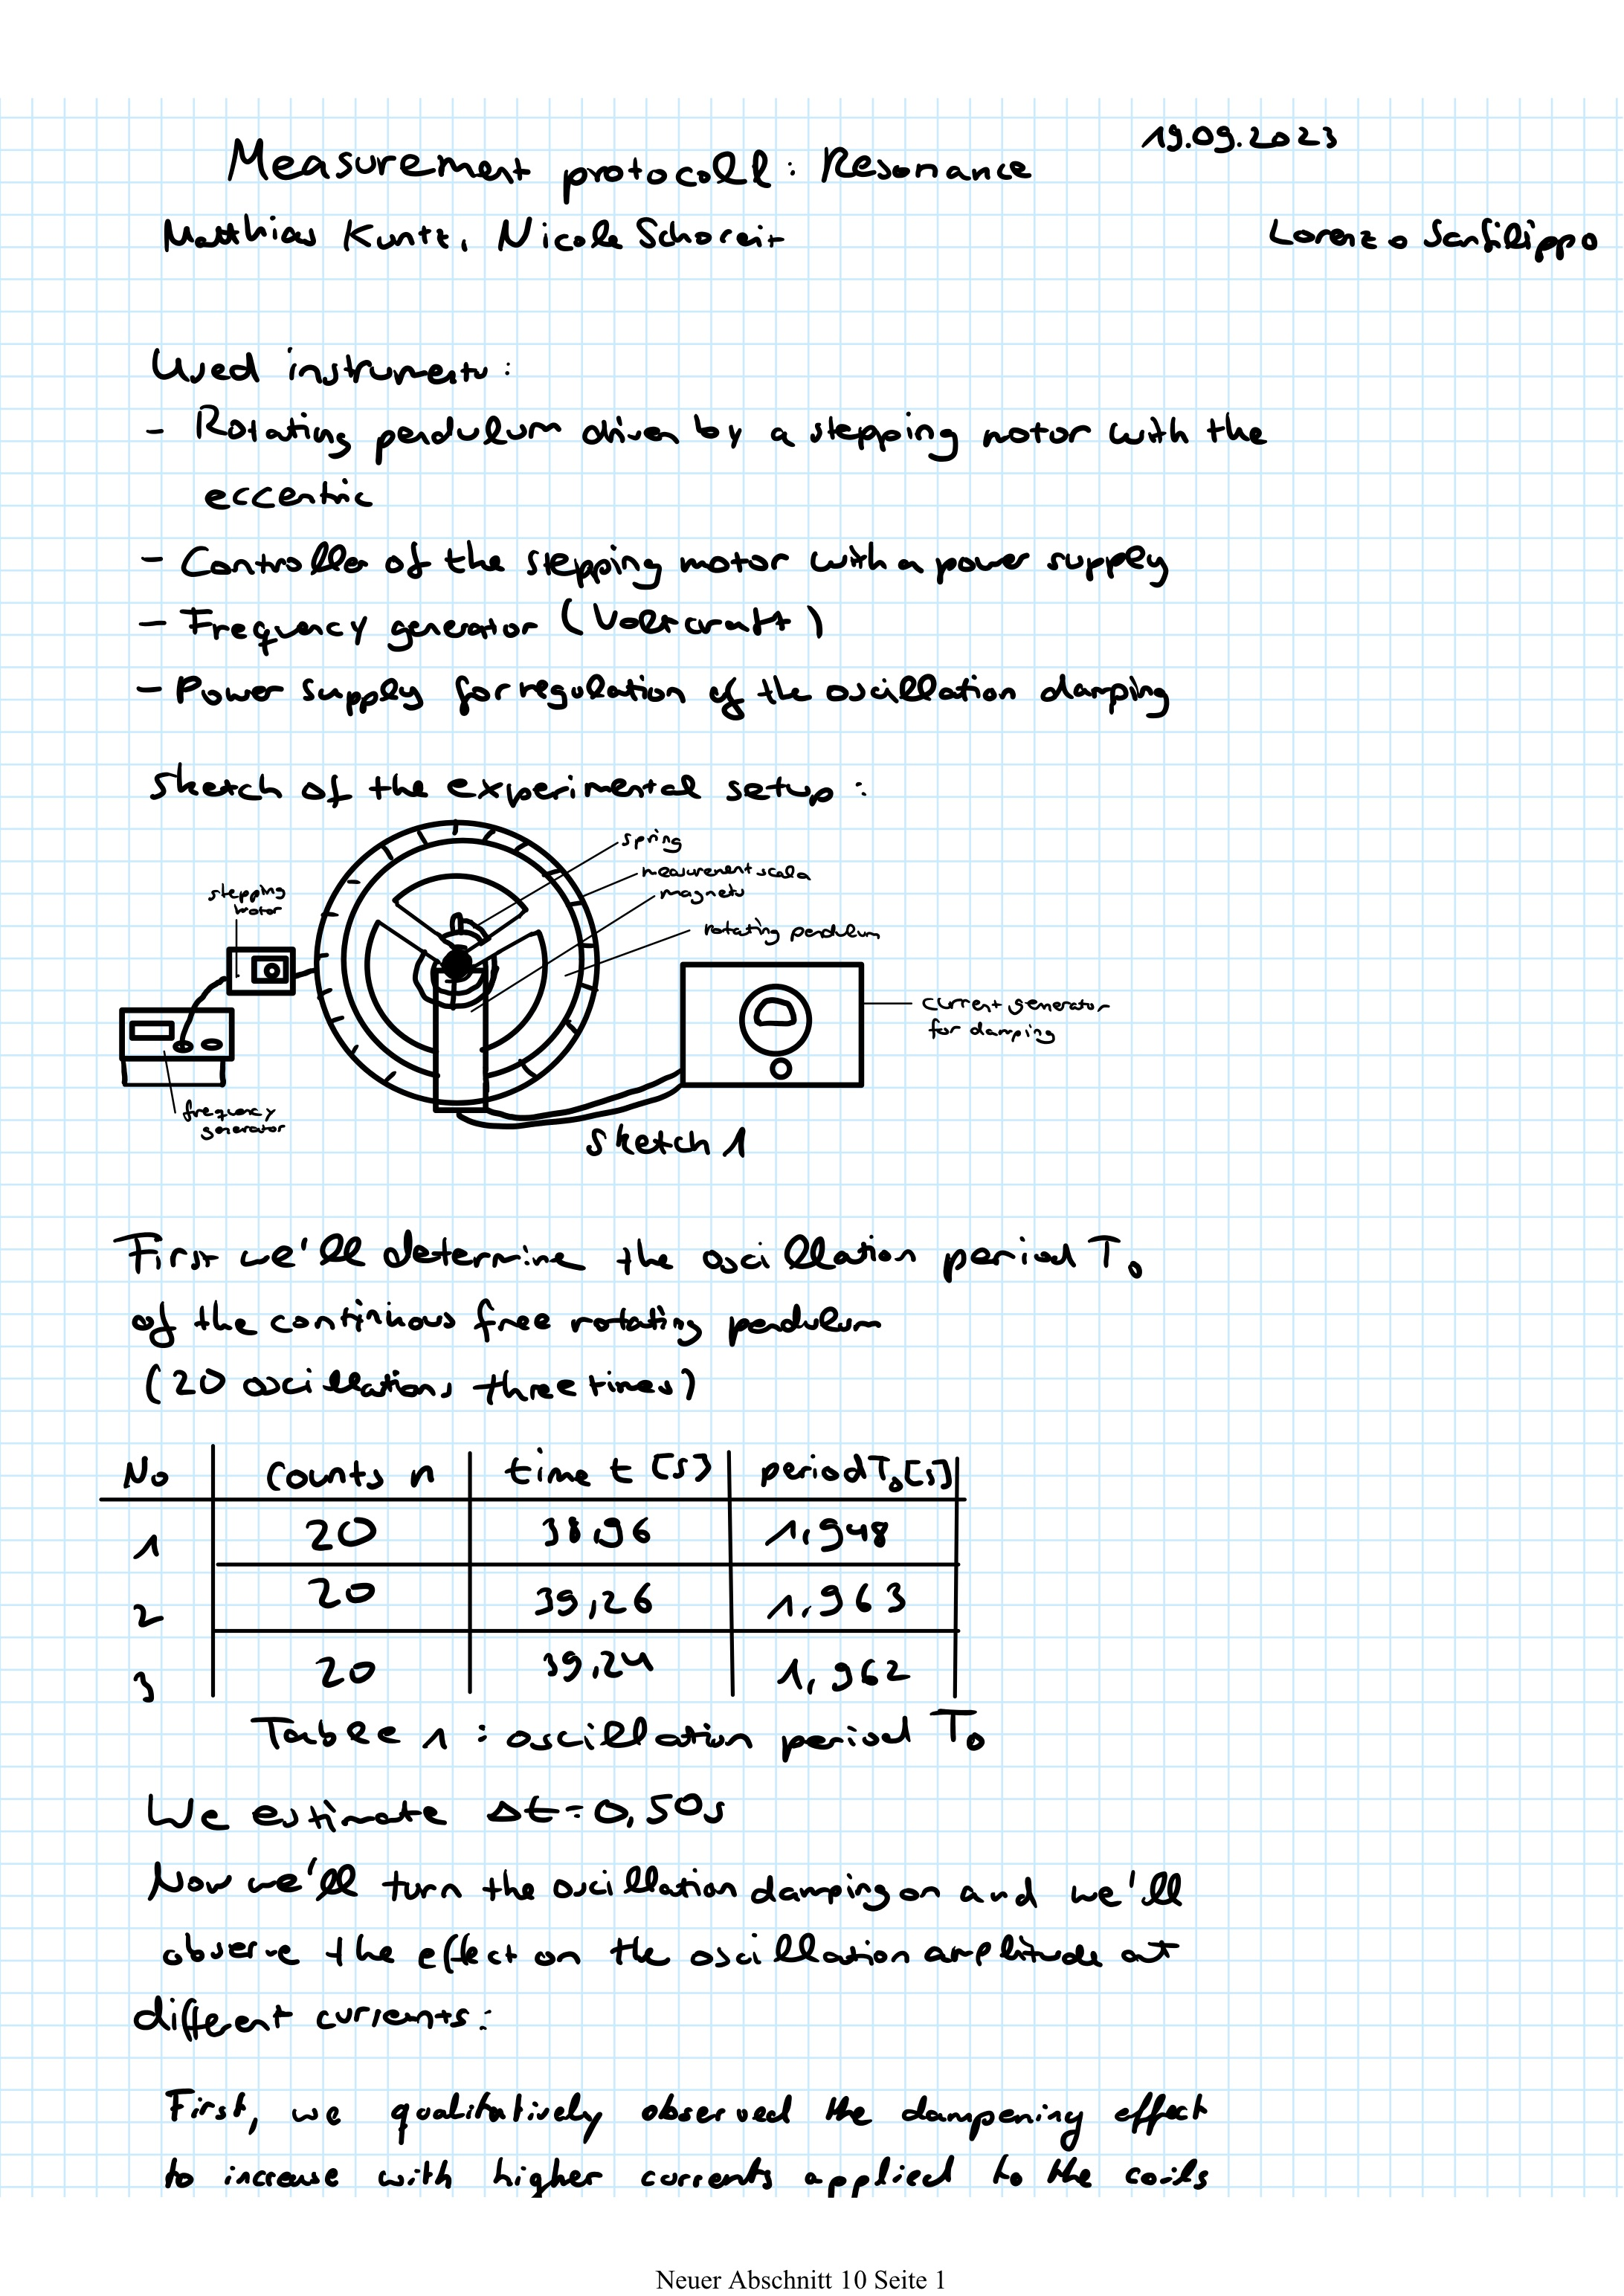
\includegraphics[width=\textwidth]{graphics/mess1.jpg}
\newpage
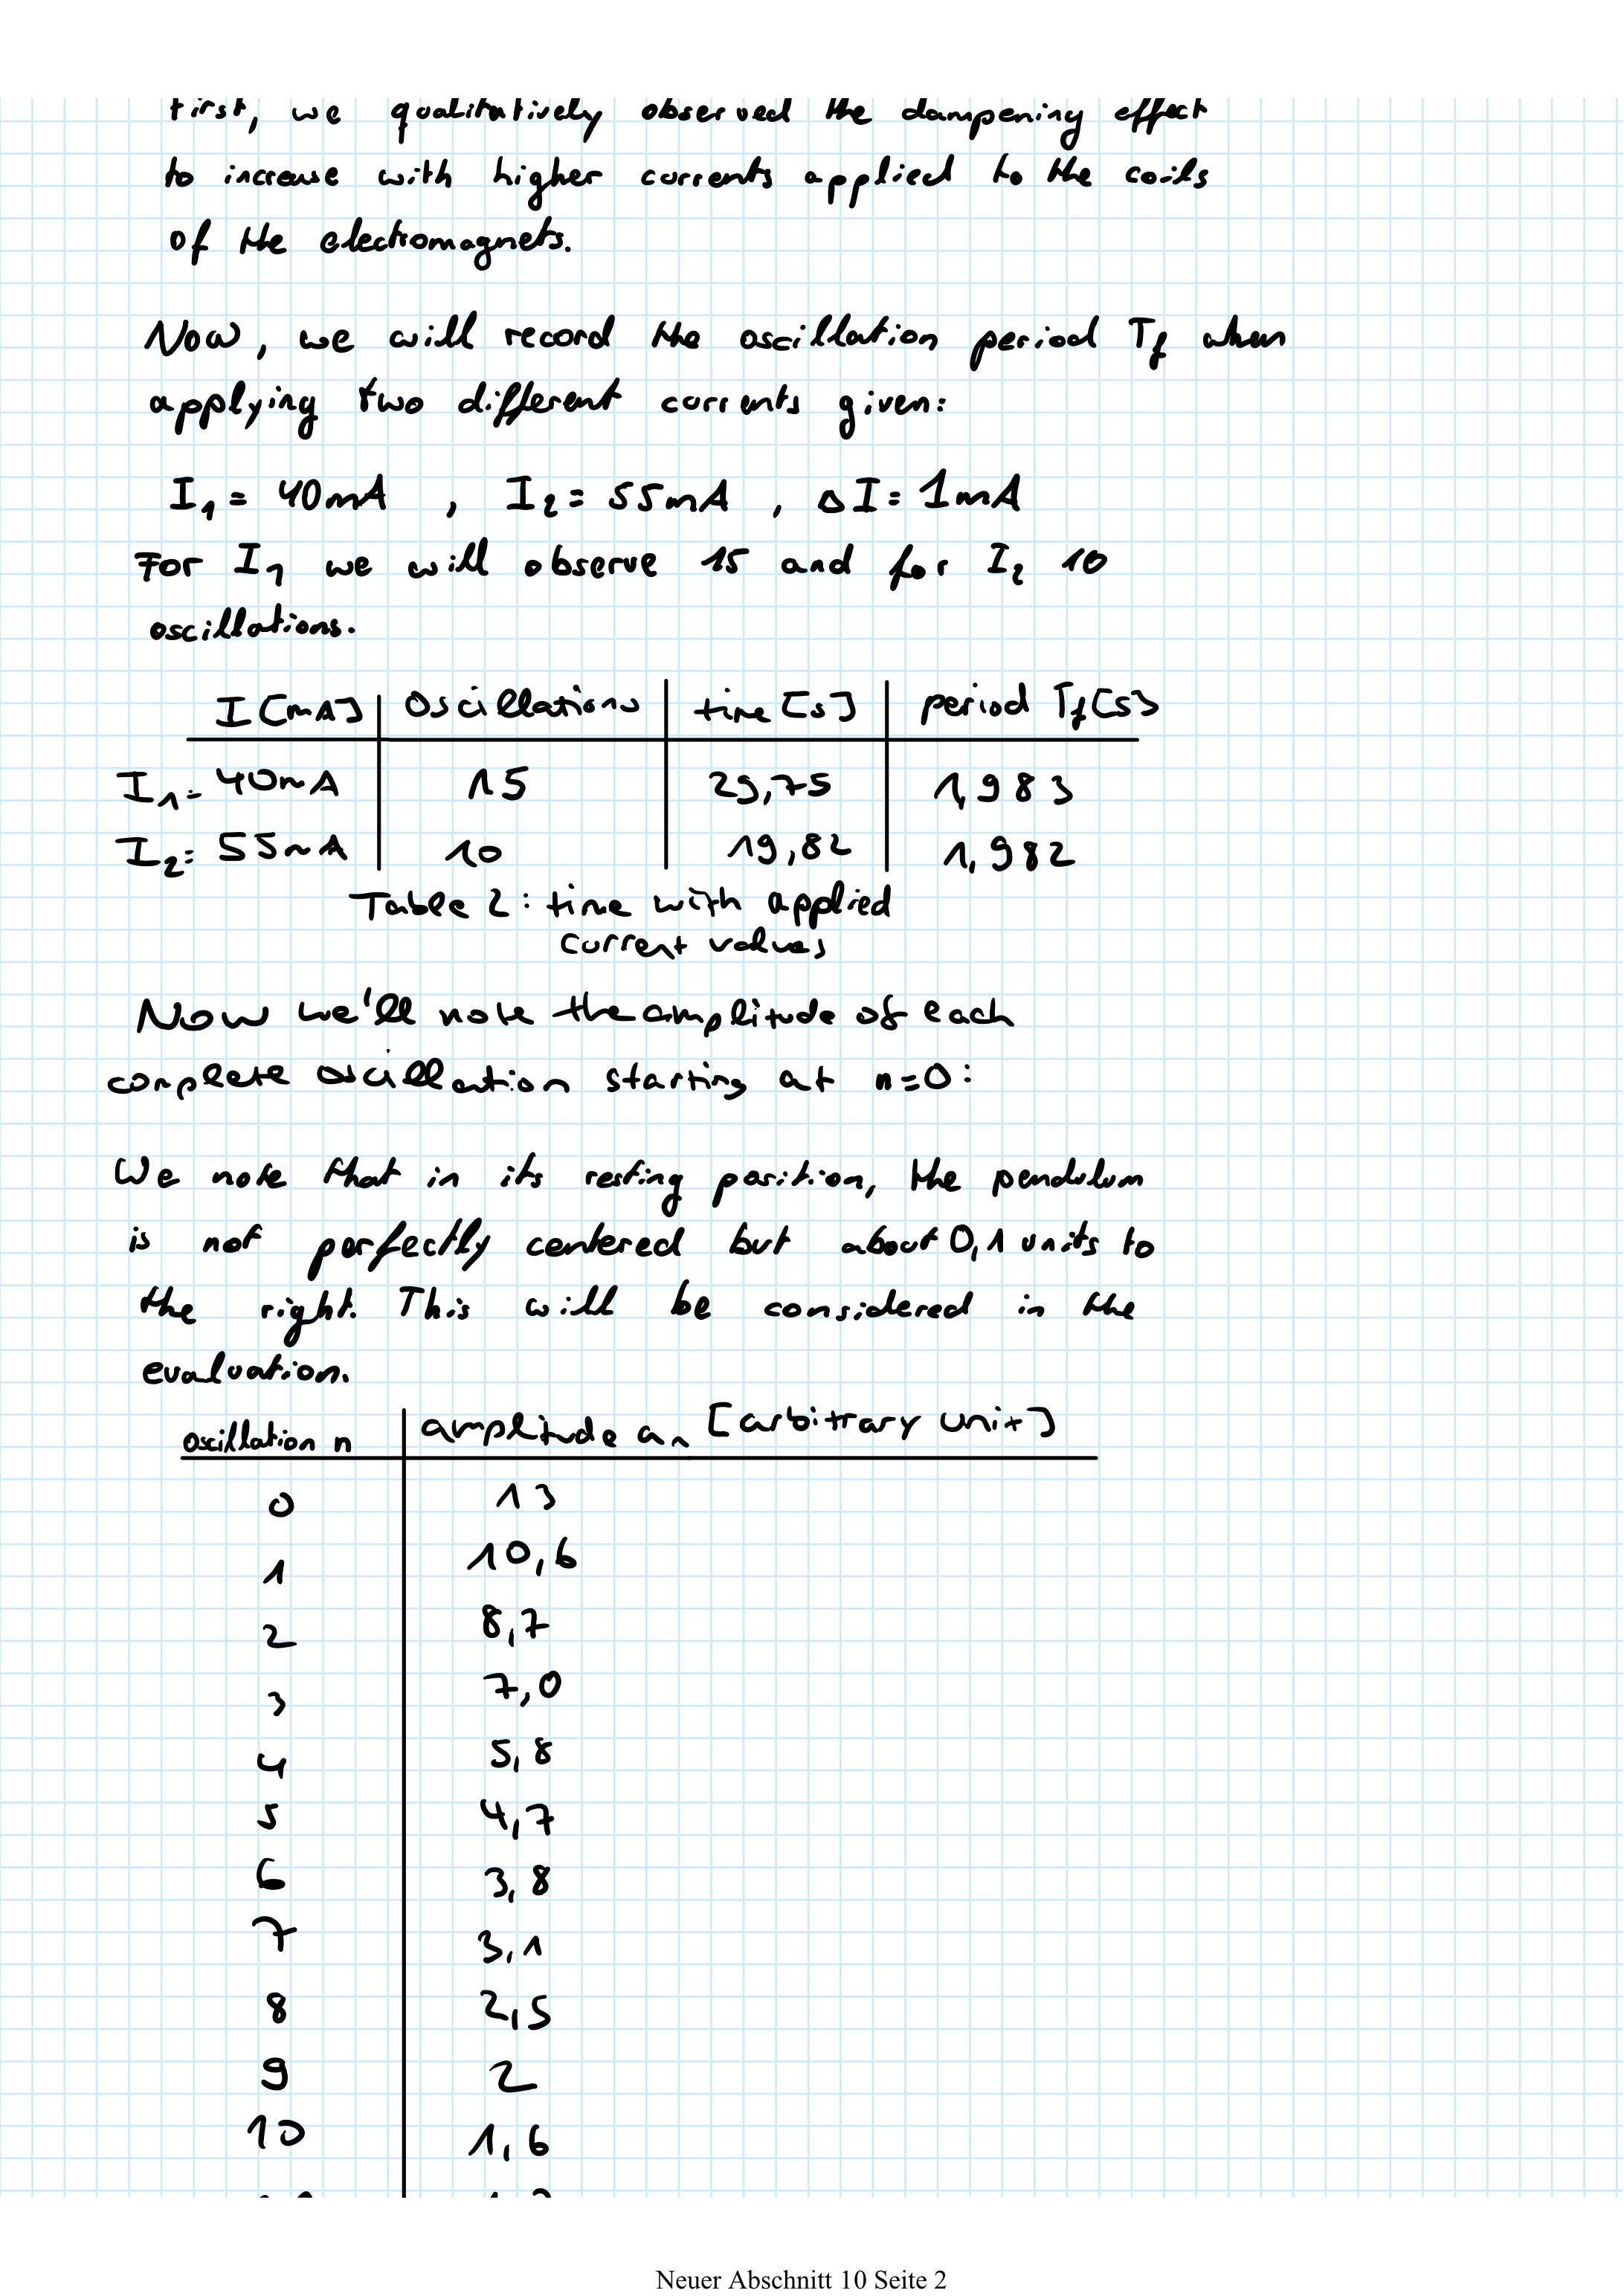
\includegraphics[width=\textwidth]{graphics/mess2.jpg}
\newpage
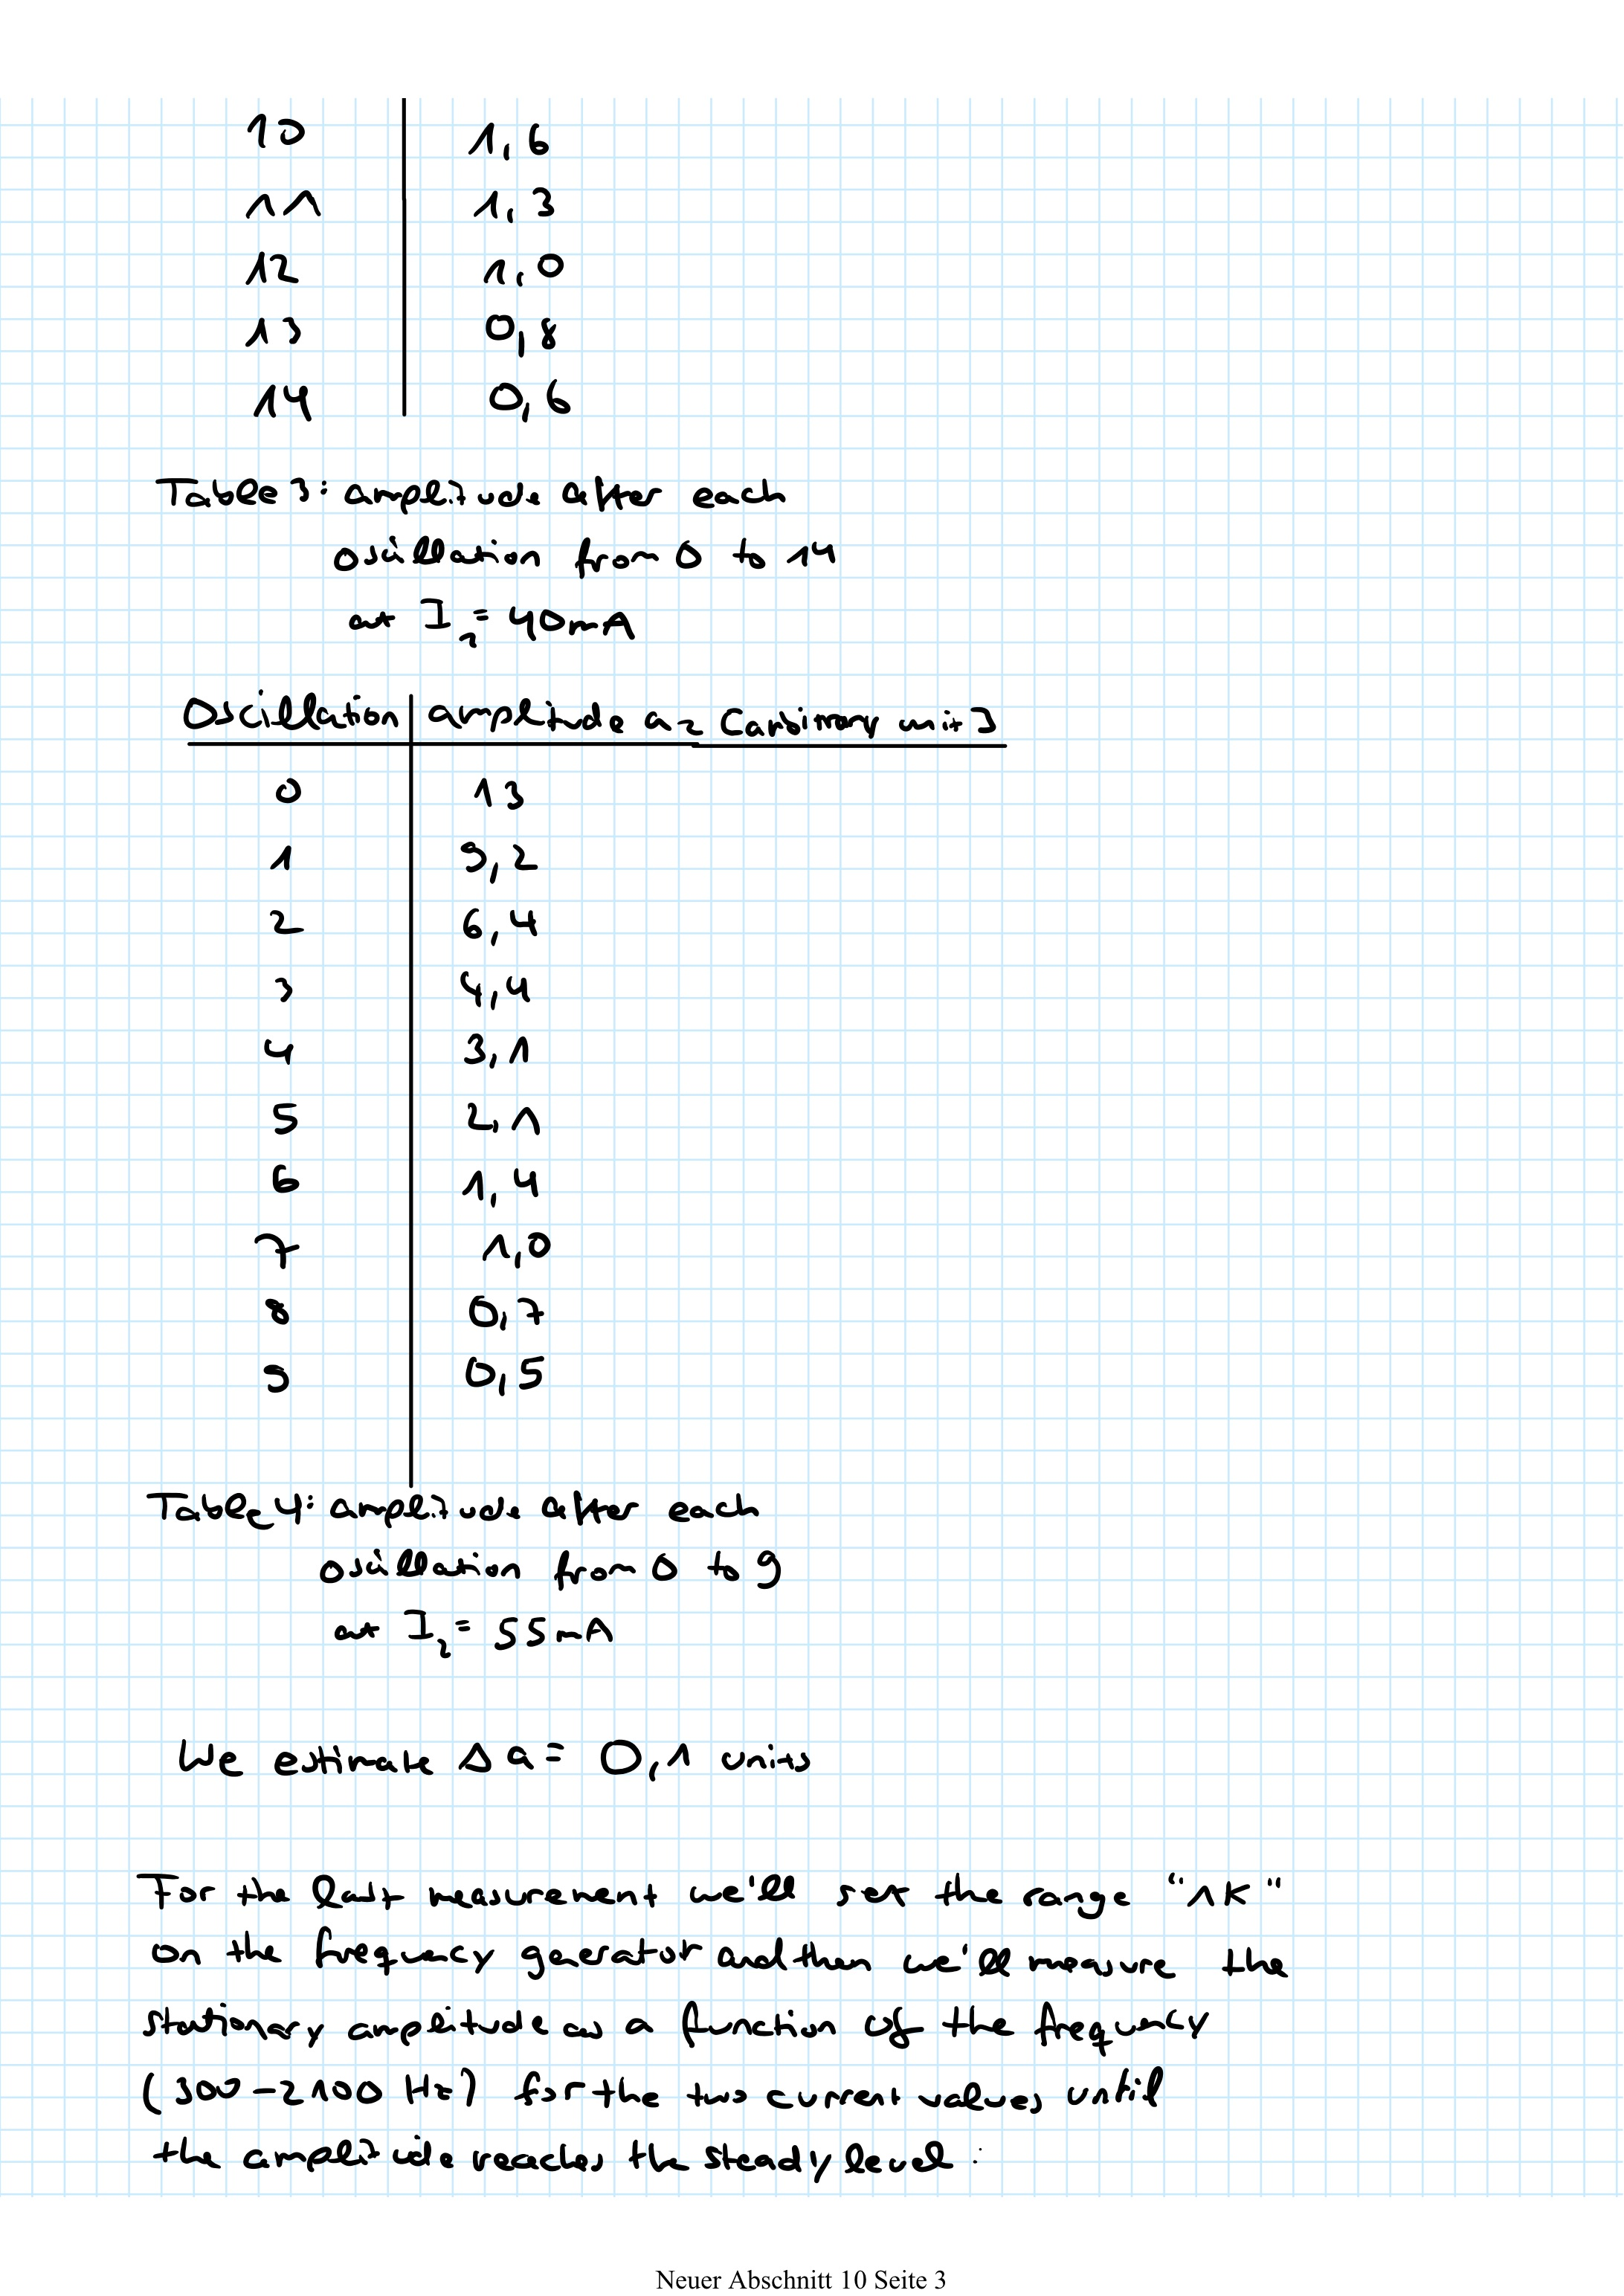
\includegraphics[width=\textwidth]{graphics/mess3.jpg}
\newpage
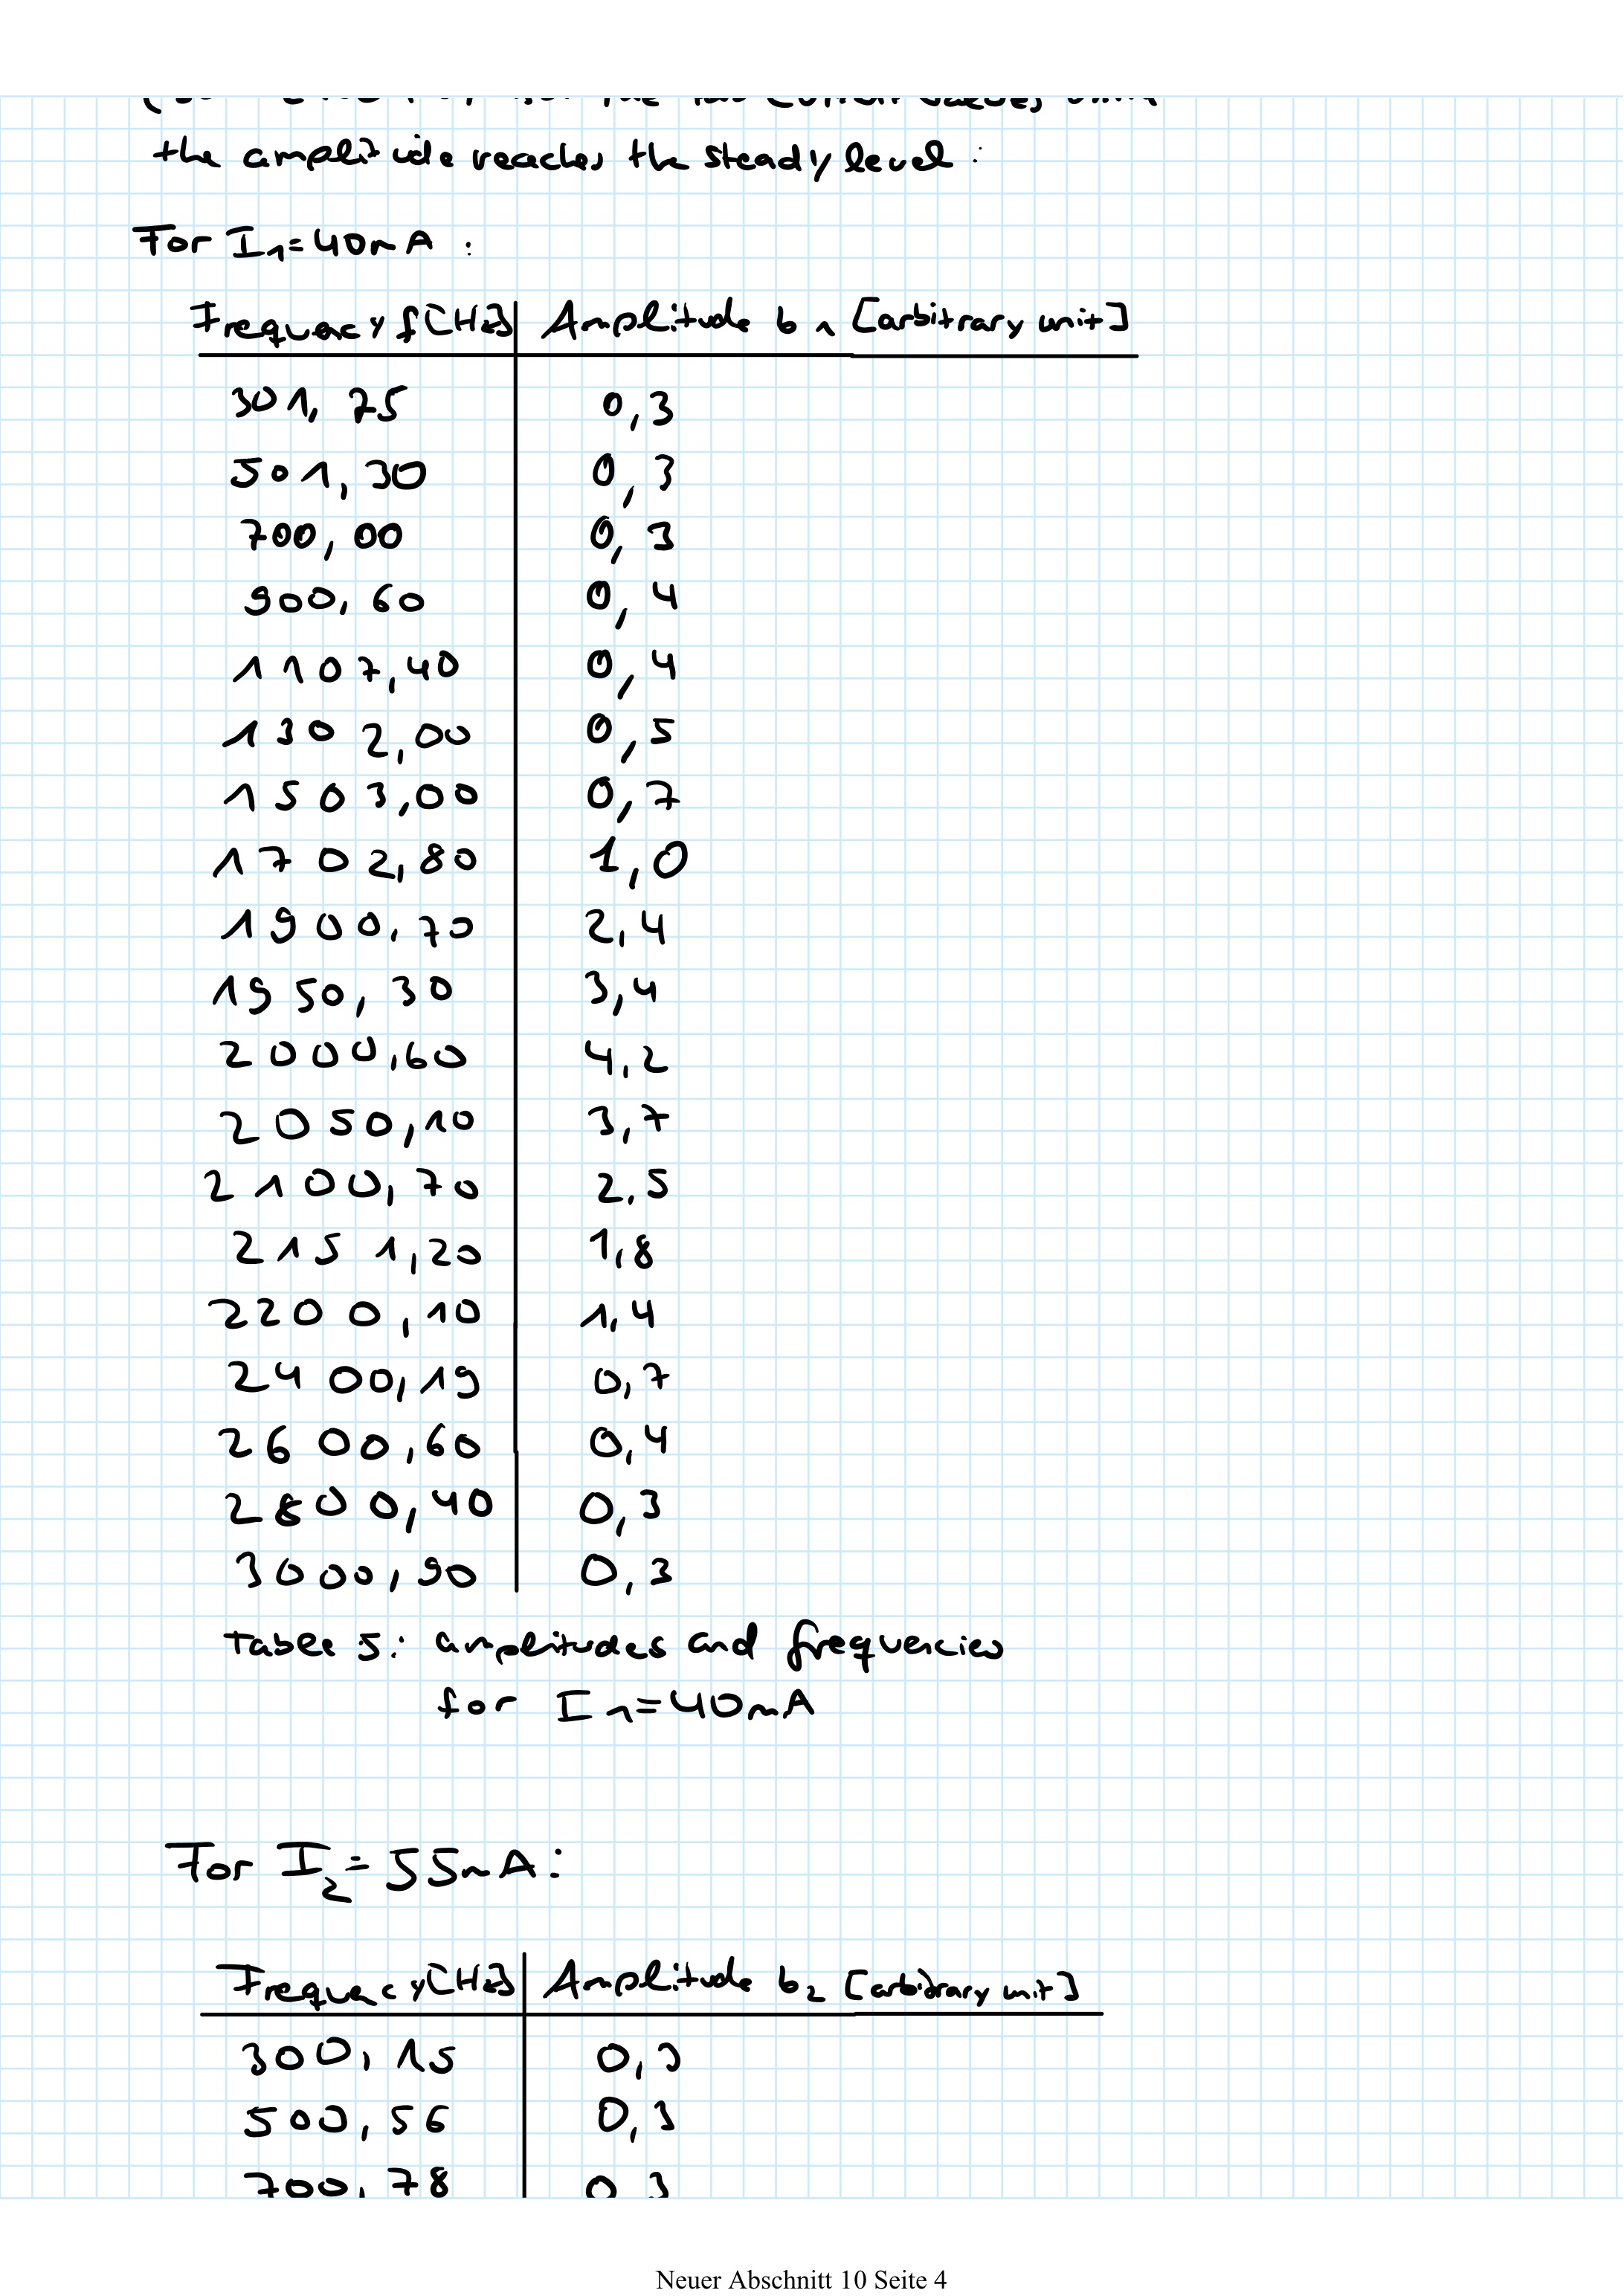
\includegraphics[width=\textwidth]{graphics/mess4.jpg}
\newpage
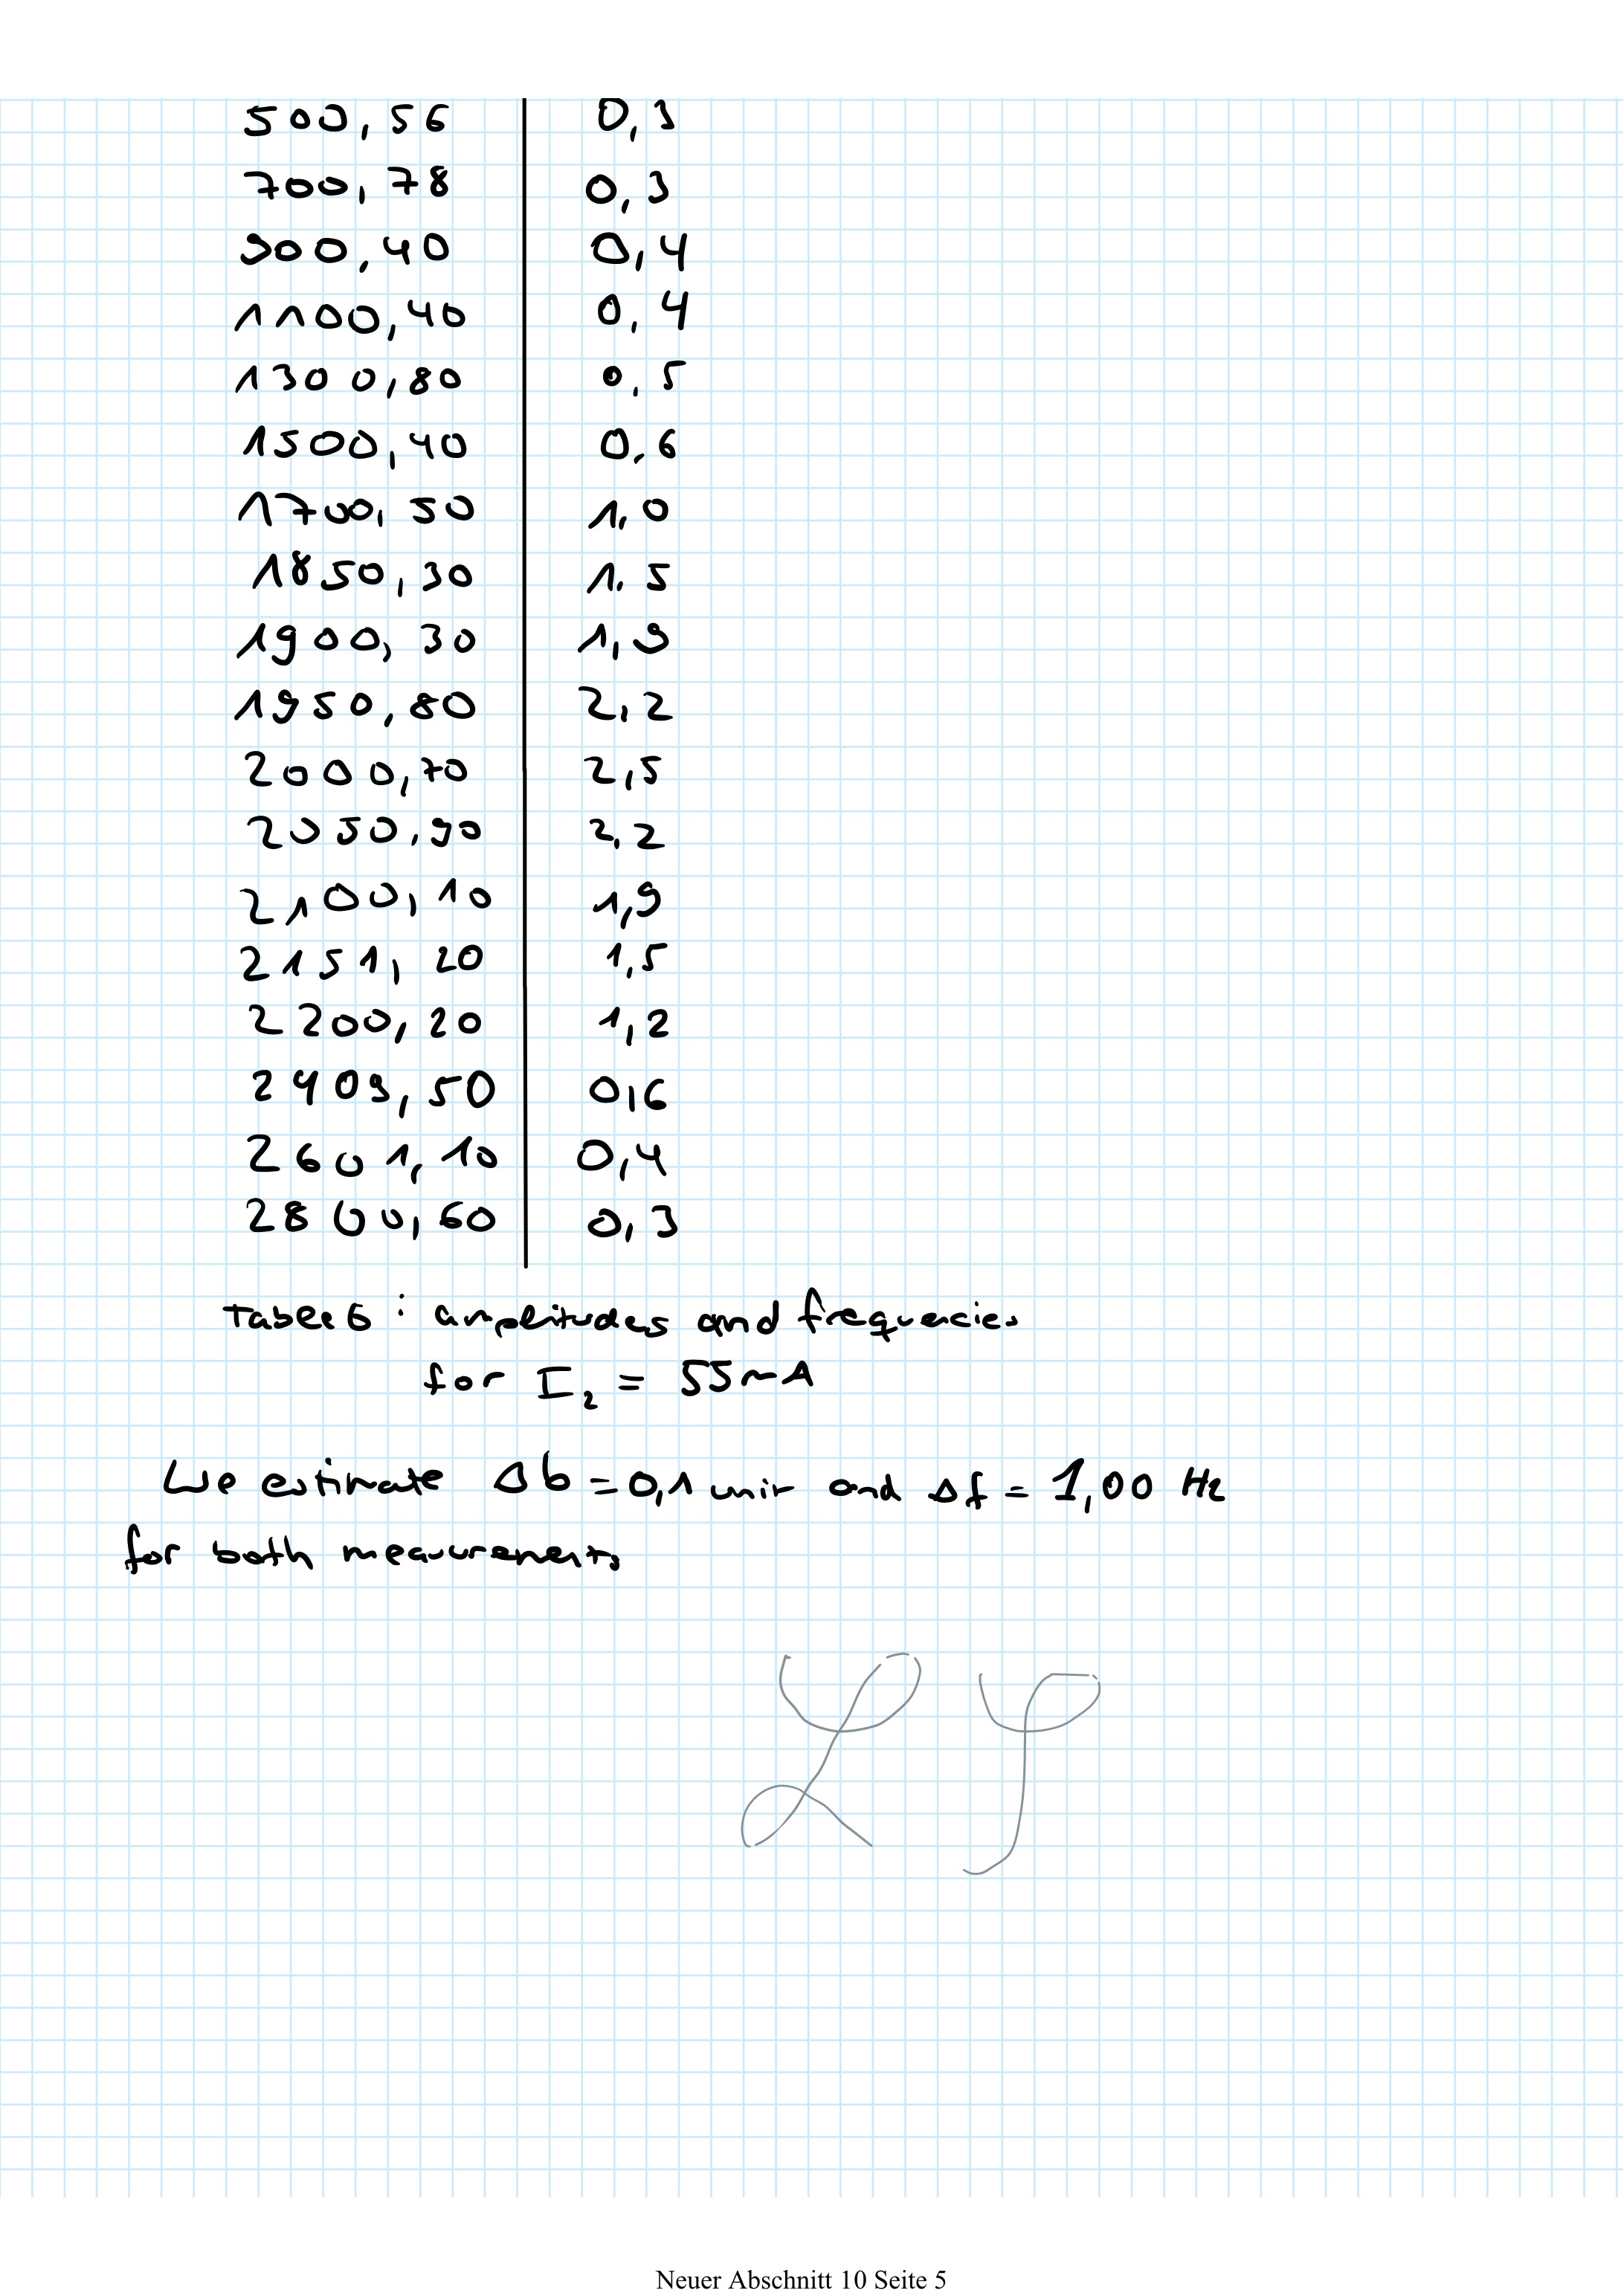
\includegraphics[width=\textwidth]{graphics/mess5.jpg}
\newpage

\addtocounter{table}{6}

%-------------------------AUSWERTUNG-------------------------
\section{Evaluation}

Firstly, we will determine the oscillation period $T_0$ of the free pendulum by taking the mean of our measured values in table 1. The error $\Delta T_0$ is calculated by quadratically adding the measurement error $\Delta t$ divided by 20 and the standard error of the mean value $\Delta T_{0_\sigma}$:

\begin{equation}
    \begin{split}
        \overline{T}_0 &= 1,958 \text{s} \\
        \Delta \overline{T}_0 &= \sqrt{\left( \frac{\Delta t}{20} \right)^2 + (\Delta T_{0_\sigma})^2} = 0,025 \text{s}\\ \\
        \implies \bm{\overline{T}_0} &= \bm{(1,958\pm0,025)} \textbf{s}
    \end{split}
    \label{eq:99}
\end{equation}

\subsection{Determining the decay constant of the dampened oscillation}

We start by plotting the amplitudes recorded in tables 3 and 4 as a function of the oscillation number in one diagram on logarithmic paper each. For both measurements, the initial amplitude was $a_0 = 12,9$ considering the mentioned error of 0,1 units, therefore we need to determine the time $t_\frac{1}{2}$ where $a(n) = 6,45$. Using equations \ref{eq:3} and \ref{eq:4} we can derive the following relations for determining $\delta$:

\begin{equation}
    \begin{split}
        t_{\frac{1}{2}_{(1)}} &= n_1 T_{f_1} \\
        t_{\frac{1}{2}_{(2)}} &= n_2 T_{f_2} \\
        \text{where} \ \ &a(n_{1/2}) = 6,45.
    \end{split}
    \label{eq:98}
\end{equation}

The indices 1 and 2 refer to the two different measurements with $I_1 = 40$mA and $I_2 = 55$mA. The oscillation periods $T_{f_1}$ and $T_{f_2}$ are taken from table 2 and their errors are the measurement errors divided by the amount of oscillations. We get:

\begin{equation}
    \begin{split}
        T_{f_1} &= (1,98 \pm 0,03) \text{s} \\
        T_{f_2} &= (1,98 \pm 0,05) \text{s} \\
    \end{split}
    \label{eq:97}
\end{equation}

From diagrams \ref{fig:1} and \ref{fig:2} we take the following values for $n_1$ and $n_2$ as well as their errors, which are estimated by how far the max-slope line deviates from the best-fit-value:

\begin{equation}
    \begin{split}
        n_1 &= 3,2 \\
        n_2 &= 1,9 \\
        \Delta n_1 &= 0,4 \\
        \Delta n_2 &= 0,2
    \end{split}
    \label{eq:96}
\end{equation}

Now we can calculate the times $t_{\frac{1}{2}_{(1)}}$ and $t_{\frac{1}{2}_{(2)}}$ using equation \ref{eq:98} and their errors using propagation:

\begin{equation}
    \begin{split}
        t_{\frac{1}{2}_{(1)}} &= 6,3 \text{s} \\
        t_{\frac{1}{2}_{(2)}} &= 3,8 \text{s} \\
        \Delta t_{\frac{1}{2}_{(1)}} &= \sqrt{(n_1 \cdot \Delta T_{f_1})^2 + (T_{f_1} \cdot \Delta n_1)^2} = 0,8 \text{s} \\
        \Delta t_{\frac{1}{2}_{(2)}} &= \sqrt{(n_2 \cdot \Delta T_{f_2})^2 + (T_{f_2} \cdot \Delta n_2)^2} = 0,4 \text{s} \\
    \end{split}
    \label{eq:95}
\end{equation}

Finally, we can determine the decay constants using equation \ref{eq:4} and propagation for the errors:

\begin{equation}
    \begin{split}
        \delta_1 &= 0,110 \text{Hz} \\
        \delta_2 &= 0,182 \text{Hz} \\ 
        \Delta \delta_1 &= \sqrt{\left( \frac{\ln{2}}{t_{\frac{1}{2}_{(1)}}^2} \cdot \Delta t_{\frac{1}{2}_{(1)}} \right)^2} = 0,014 \text{Hz} \\
        \Delta \delta_2 &= \sqrt{\left( \frac{\ln{2}}{t_{\frac{1}{2}_{(2)}}^2} \cdot \Delta t_{\frac{1}{2}_{(2)}} \right)^2} = 0,019 \text{Hz} \\ \\
        \implies \bm{\delta_1} &= \bm{(0,110 \pm 0,014)} \textbf{Hz} \\
        \bm{\delta_2} &= \bm{(0,182 \pm 0,019)} \textbf{Hz} \\
    \end{split}
    \label{eq:94}
\end{equation}

\begin{figure} [p]
    \centering
    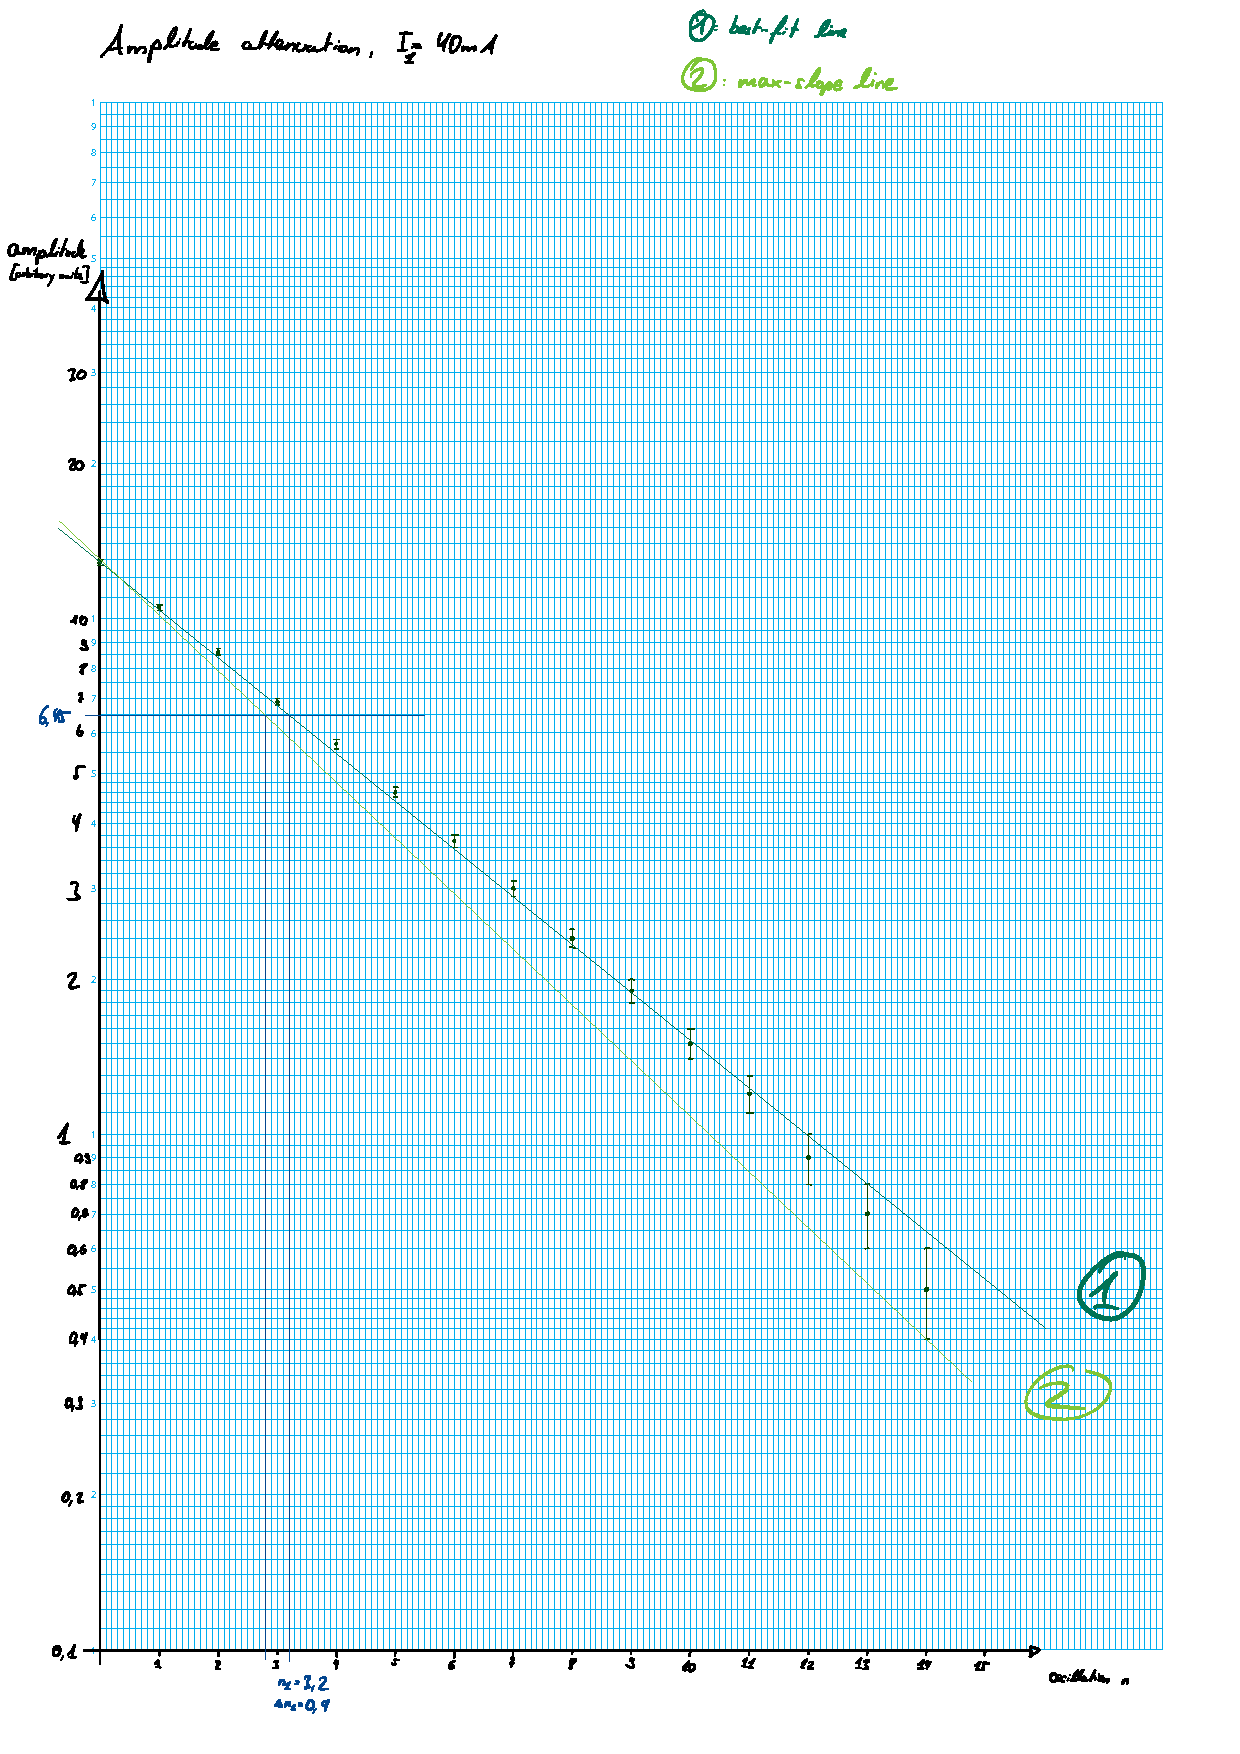
\includegraphics[width=\textwidth]{graphics/13-dia1.pdf}
    \caption{Amplitude attenuation with $I_1 = 40$mA}
    \label{fig:1}
\end{figure}

\begin{figure} [p]
    \centering
    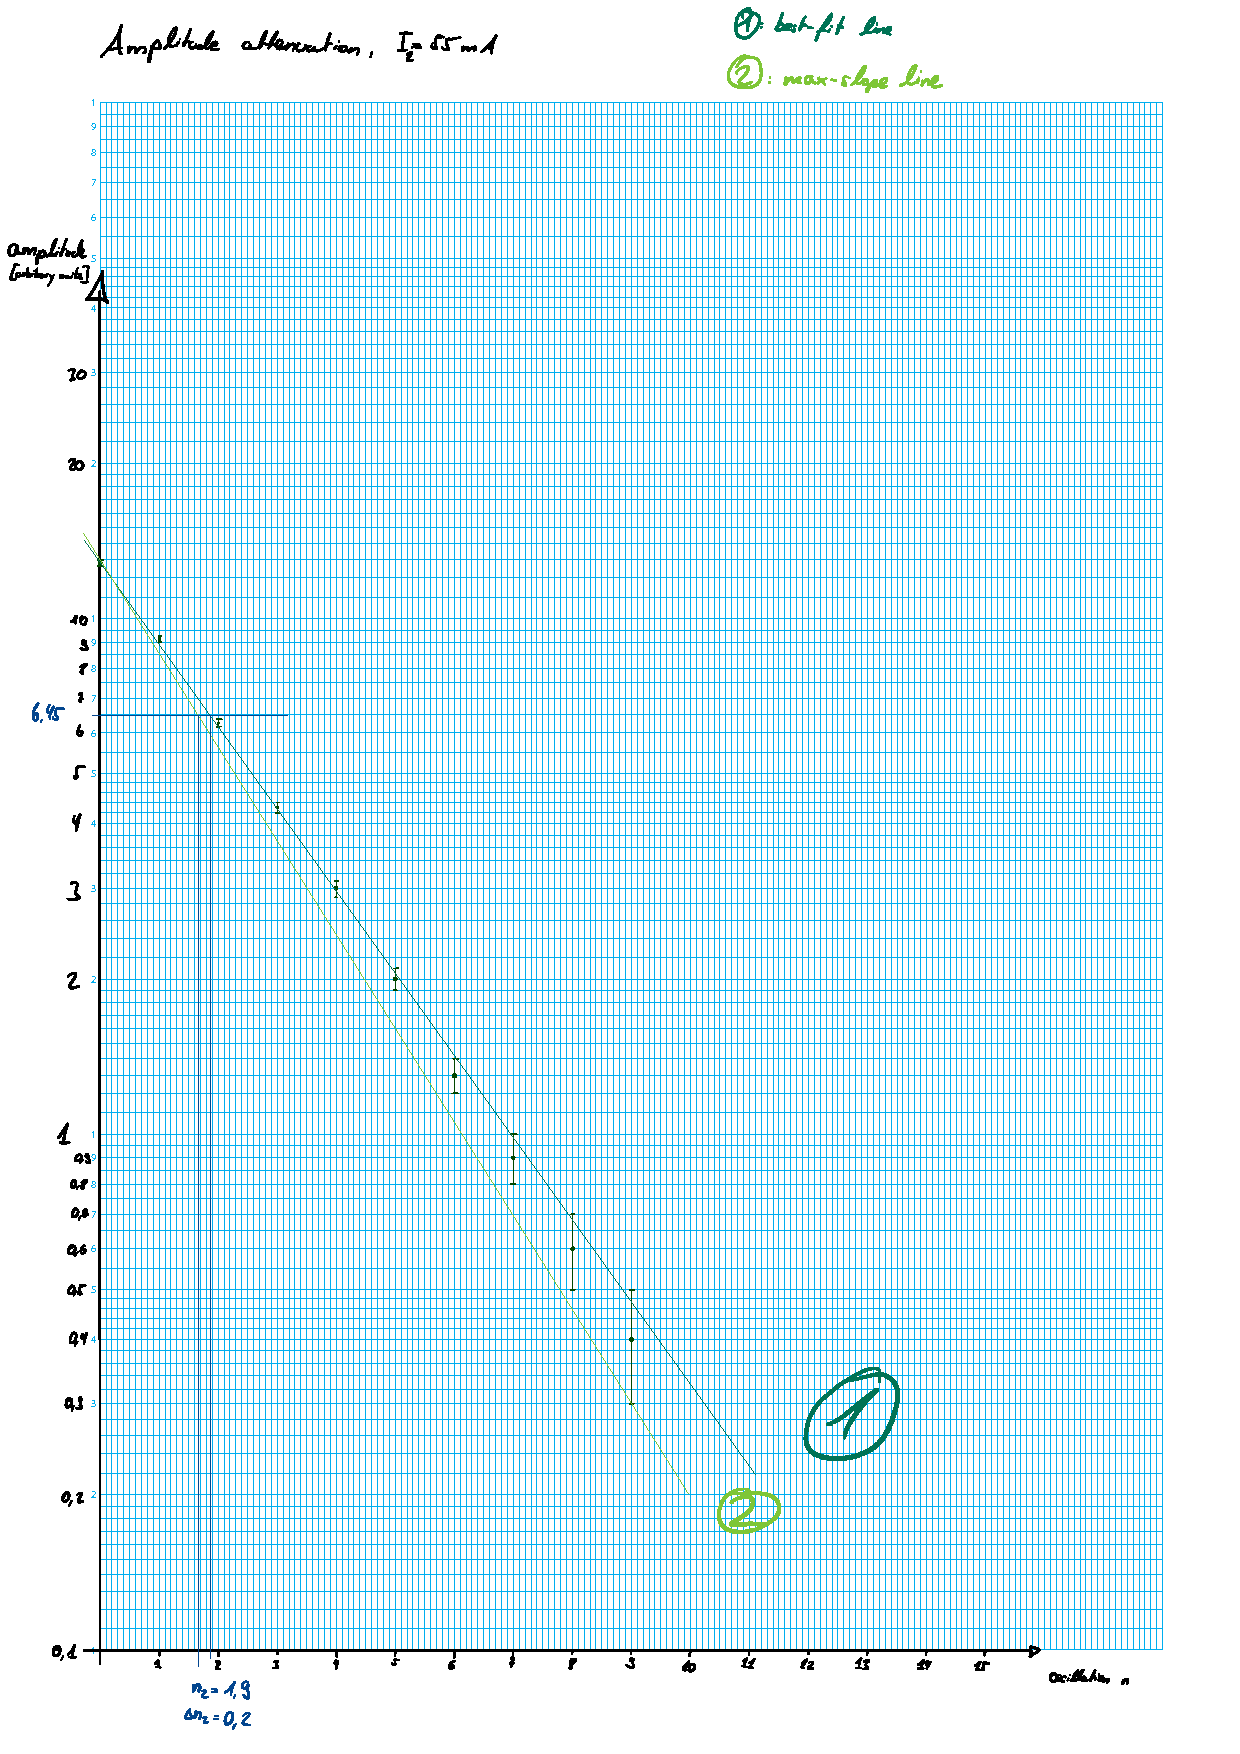
\includegraphics[width=\textwidth]{graphics/13-dia2.pdf}
    \caption{Amplitude attenuation with $I_2 = 55$mA}
    \label{fig:2}
\end{figure}

\newpage

\subsection{Determining the decay constant of the stimulated oscillation}

We start by plotting the amplitude of the stimulated oscillation as a function of the driving generator frequency. It is important to note, that we first need to calculate the generated frequency of the generator to the actual frequency of the stepping motor. Their relation was given 1:4000. The effective angular frequencies are therefore

\begin{equation}
    \begin{split}
        \omega &= 2\pi \frac{f}{4000}, \\
        \Delta \omega &= 2\pi \frac{\Delta f}{4000}.
    \end{split}
    \label{eq:93}
\end{equation}

For simplicity's sake we made the diagram using the frequencies given in tables 5 and 6 and only calculated the relevant angular frequencies. The diagrams are shown in figures \ref{fig:3} and \ref{fig:4}. We determine these values and estimate the error $\Delta f = 25$Hz based on the accuracy of our drawing skills and the estimated trajectory between the inserted points.

First, we determine the frequency at the resonance peaks:

\begin{equation}
    \begin{split}
        \omega_1 &= (3,16 \pm 0,04) \text{Hz} \\
        \omega_2 &= (3,14 \pm 0,04) \text{Hz} \\
    \end{split}
    \label{eq:92}
\end{equation}

We compare these angular frequencies to the eigenfrequencies of the pendulum $\omega_e$ for each of the currents calculated from the oscillation periods $T_f$ recorded in table 2. The errors $\Delta T_f$ are again determined as $\Delta t$ divided by the number of oscillations:

\begin{equation}
    \begin{split}
        \omega_e &= \frac{2\pi}{T_{f}} \\ 
        \Delta \omega_e &= \sqrt{\left( \frac{2\pi}{T_{f}^2} \cdot \Delta T_f \right)^2} \\ \\
        \omega_{e_1} &= (3,17 \pm 0,05) \text{Hz} \\
        \omega_{e_2} &= (3,17 \pm 0,08) \text{Hz} \\        
    \end{split}
\end{equation}

\newpage

The comparison yields:

\begin{equation}
    \begin{split}
        \sigma &= \frac{|\omega - \omega_e|}{\sqrt{(\Delta \omega)^2 + (\Delta \omega_e)^2}} \\ \\
        \sigma_1 &= 0,16 \\
        \sigma_2 &= 0,34 
    \end{split}
\end{equation}

As we can see, the deviation is insignificant, so the frequencies of the resonance peaks overlap with the eigenfrequencies.

\bigskip

\textbf{Method 1: the half-width}

The first method of determining the decay constant is by first calculating the half-width of each graphs. For this, we will find the two frequencies at which the amplitude is $\frac{1}{\sqrt{2}}$-times the maximum amplitude and use equation \ref{eq:8} to first calculate the half width $H$ and then the decay constant $\delta$ as well as its error using propagation:

\begin{equation}
    \Delta \delta = \sqrt{\left( \frac{\Delta H}{2} \right)^2}.
    \label{eq:91}
\end{equation}

We get the results shown in table \ref{tab:1}.

\begin{table} [!ht]
    \centering
    \caption{calculating the decay constant via the half-width}
    \bigskip
    \resizebox{\textwidth}{!}{
    \begin{tabular}{cccccccc}
        \hline
        $\bm{I}$ [mA] & $\bm{f_1}$ [Hz] & $\bm{f_2}$ [Hz] & $\bm{\Delta f_{1/2}}$ [Hz] & $\bm{H}$ [Hz] & $\bm{\Delta H}$ [Hz] & $\bm{\delta}$ [Hz] & $\bm{\Delta \delta}$ [Hz] \\ \hline
        40 & 1920 & 2080 & 25 & 0,25 & 0,06 & 0,13 & 0,03 \\
        55 & 1885 & 2115 & 25 & 0,36 & 0,06 & 0,18 & 0,03 \\ \hline
    \end{tabular}}
    \label{tab:1}
\end{table}

\begin{equation}
    \begin{split}
        \bm{\delta_1} = \bm{(0,13 \pm 0,03)} \textbf{Hz} \\
        \bm{\delta_2} = \bm{(0,18 \pm 0,03)} \textbf{Hz} \\
    \end{split}
\end{equation}

\newpage

\textbf{Method 2: the resonance ratio}

The second method of calculating $\delta$ is via equation \ref{eq:9}, the resonance ratio. For this we need the undampened oscillation period $\omega_0$ as well as the two values $b(\omega')$ and $b(\omega \rightarrow 0)$. For $\omega_0$ we take our results from equation \ref{eq:99}:

\begin{equation}
    \begin{split}
        \omega_0 &= \frac{2\pi}{\overline{T}_0} = 3,21 \frac{\text{rad}}{\text{s}}\\
        \Delta \omega_0 &= \sqrt{\left( \frac{2\pi}{\overline{T}_0^2} \cdot \Delta \overline{T}_0 \right)^2} = 0,04 \frac{\text{rad}}{\text{s}}\\
    \end{split}
\end{equation}

The values $b(\omega')$ and $b(\omega \rightarrow 0)$ are determined from diagrams \ref{fig:3} \& \ref{fig:4} and for their errors we take the amplitude error of $\Delta b = 0,1$. With everything needed together we can calculate the decay constant using equation \ref{eq:9} and its error using error propagation:


\begin{equation}
    \begin{split}
        \delta &= \frac{\omega_0}{2} \frac{b(\omega \rightarrow 0)}{b(\omega')} \\
        \Delta \delta &= \sqrt{\left( \frac{b(\omega \rightarrow 0)}{2b(\omega')} \cdot \Delta \omega_0 \right)^2 + \left( \frac{\omega_0}{2b(\omega')} \cdot \Delta b(\omega \rightarrow 0) \right)^2 + \left( \frac{\omega_0}{2b(\omega')^2} \cdot \Delta b(\omega') \right)^2}
    \end{split}
\end{equation}

The results are shown in table \ref{tab:2}.

\begin{table} [!ht]
    \centering
    \caption{calculating the decay constant via equation \ref{eq:9}}
    \bigskip
    \begin{tabular}{ccccc}
        \hline
        $\bm{I}$ [mA] & $\bm{b(\omega')}$ [Hz] & $\bm{b(\omega \rightarrow 0)}$ [Hz] & $\bm{\delta'}$ [Hz] & $\bm{\Delta \delta'}$ [Hz] \\ \hline
        40 & 4,3 & 0,3 & 0,11 & 0,04 \\
        55 & 2,5 & 0,3 & 0,19 & 0,07 \\ \hline
    \end{tabular}
    \label{tab:2}
\end{table}

\begin{equation}
    \begin{split}
        \bm{\delta'_1} = \bm{(0,11 \pm 0,04)} \textbf{Hz} \\
        \bm{\delta'_2} = \bm{(0,19 \pm 0,07)} \textbf{Hz} \\
    \end{split}
\end{equation}

\newpage

We can now compare the determined values for the decay constant from method 1 $\delta$ and method 2 $\delta'$:

\begin{equation}
    \begin{split}
        \sigma &= \frac{|\delta' - \delta|}{\sqrt{(\Delta \delta')^2+(\Delta \delta)^2}} \\ \\
        \sigma_1 &= 0,4 \\
        \sigma_2 &= 0,13 \\
    \end{split}
\end{equation}

As we can see, the deviations are insignificant.

\begin{figure} [p]
    \centering
    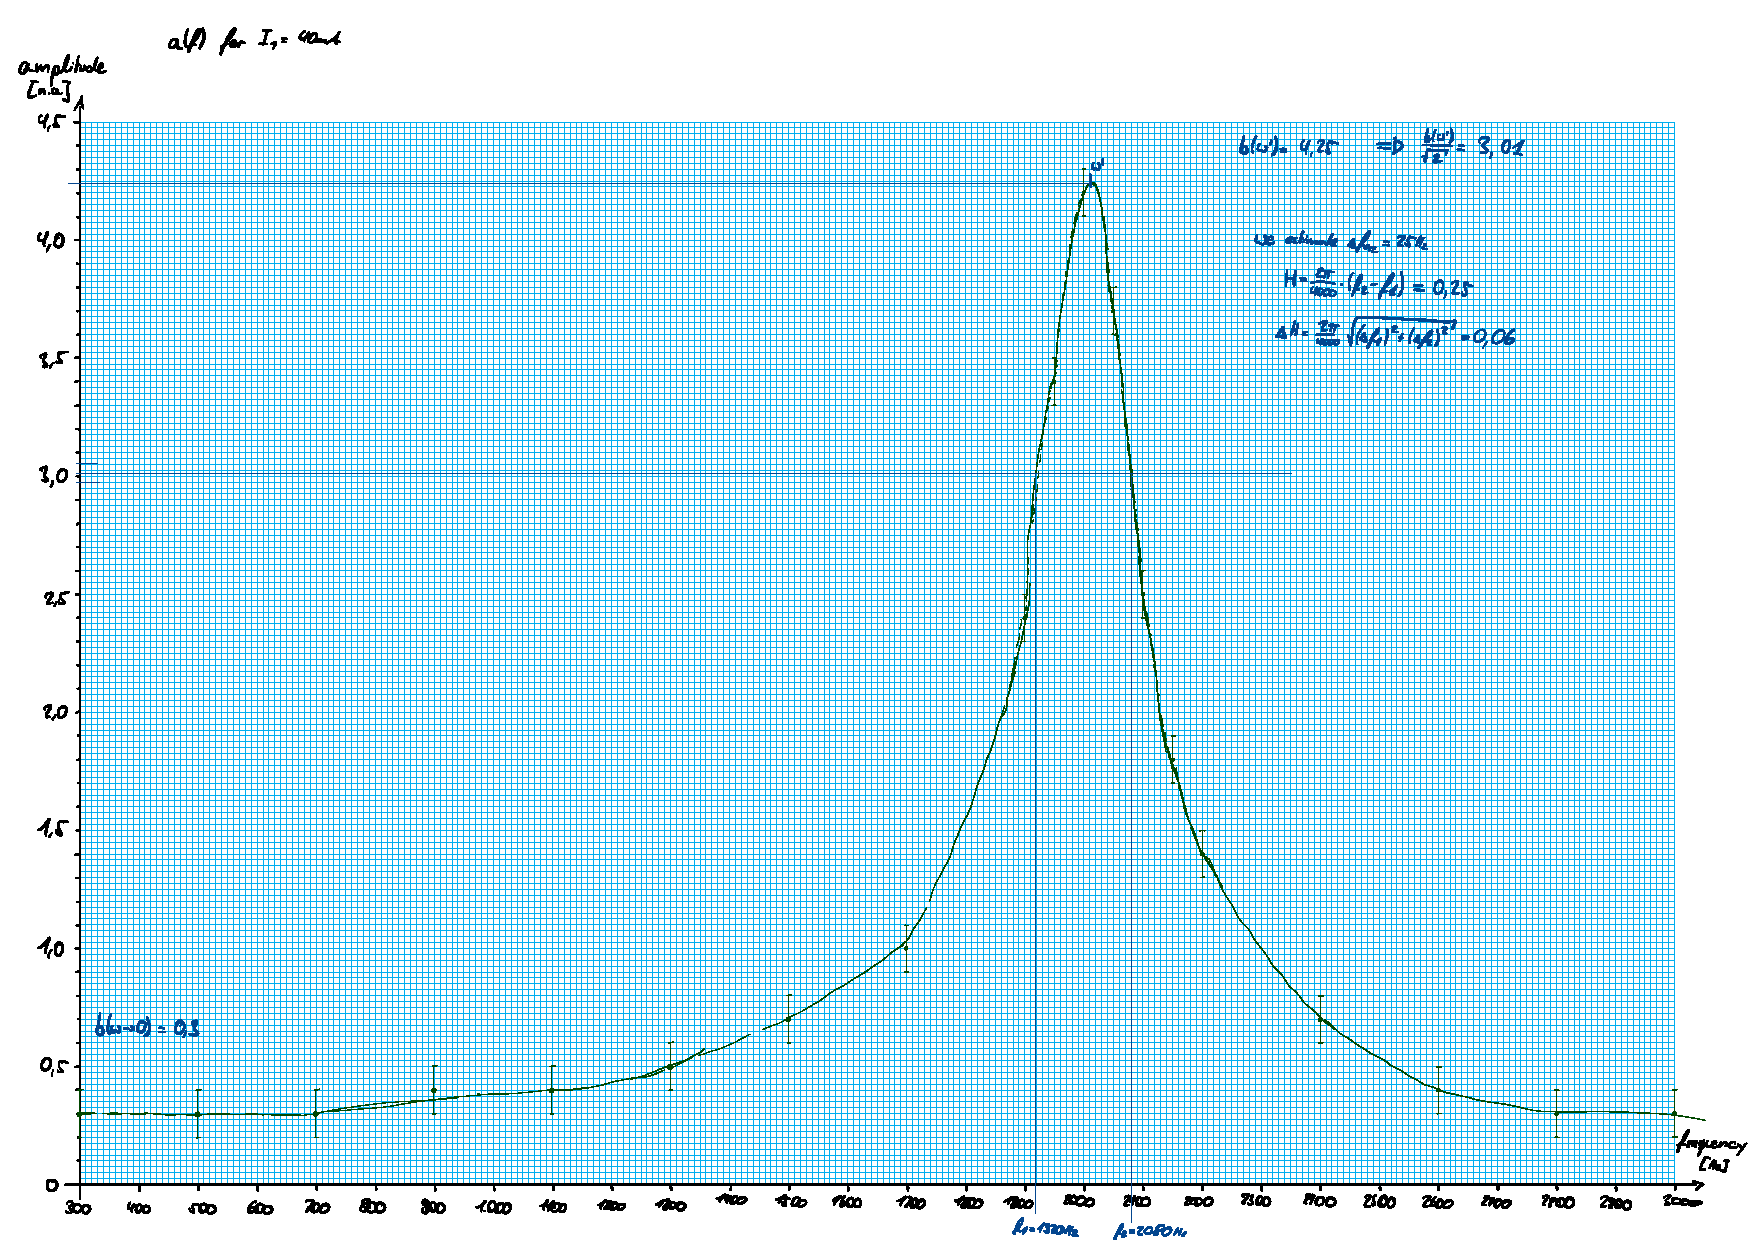
\includegraphics[height=\textwidth, angle=90]{graphics/13-dia3.pdf}
    \caption{Resonance curve for the stimulated oscillation with $I_1 = 40$mA}
    \label{fig:3}
\end{figure}

\begin{figure} [p]
    \centering
    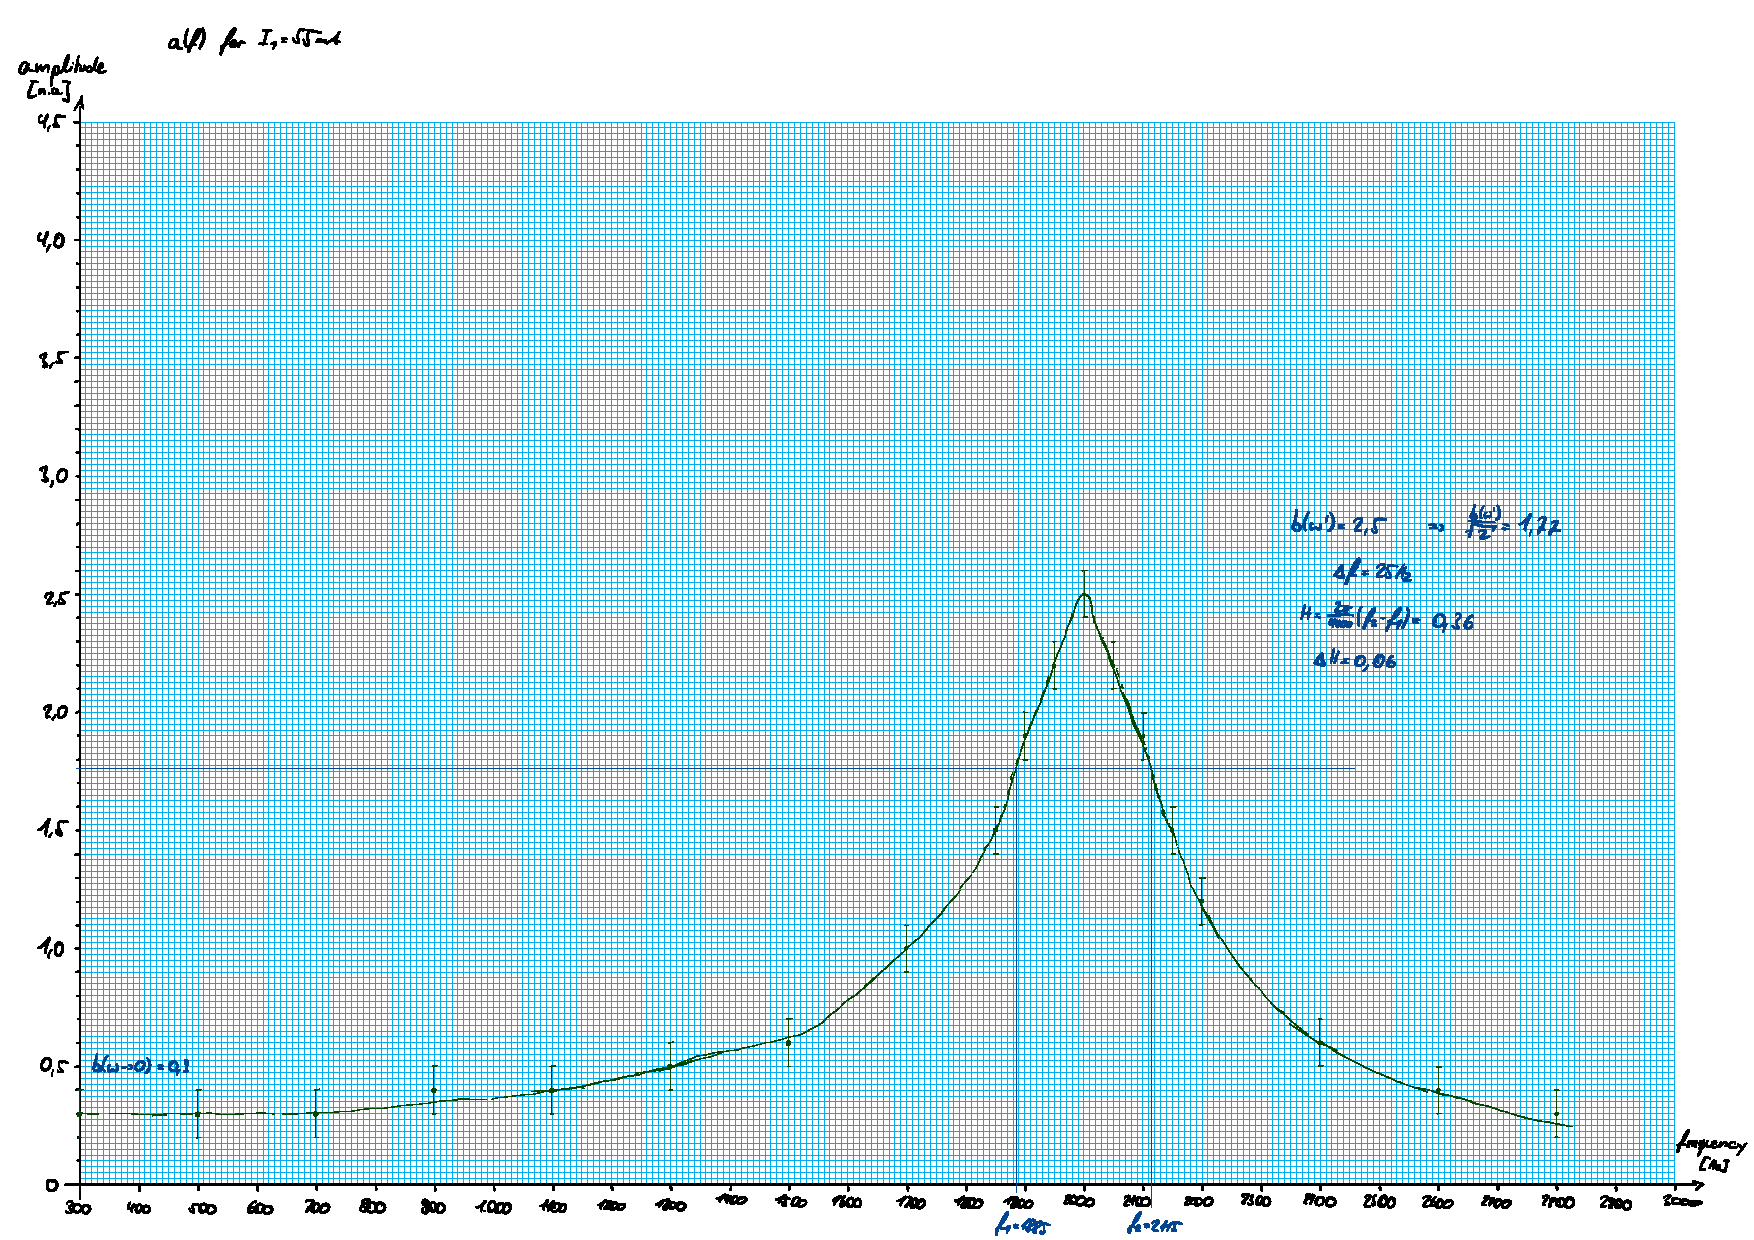
\includegraphics[height=\textwidth, angle=90]{graphics/13-dia4.pdf}
    \caption{Resonance curve for the stimulated oscillation with $I_2 = 55$mA}
    \label{fig:4}
\end{figure}


\newpage
%---------------PRÄSENTATION DER ENDERGEBNISSE---------------
\section{Presentation of final results}

In this experiment we first determined the oscillation period of the free pendulum: 

\begin{equation}
    \bm{\overline{T}_0} = \bm{(1,958\pm0,025)} \textbf{s}
\end{equation}

Then we calculated the decay constant of the dampened oscillation using different currents for the electromagnetic coils acting as brakes:

\begin{equation}
    \begin{split}
        \bm{\delta_1} &= \bm{(0,110 \pm 0,014)} \textbf{Hz} \\
        \bm{\delta_2} &= \bm{(0,182 \pm 0,019)} \textbf{Hz} 
    \end{split}
\end{equation}

Finally, we determined the decay constants of the stimulated oscillation again with different currents applied to the brakes in two different ways. The results were within insignificant differences:

\begin{equation}
    \begin{split}
        \bm{\delta_1} = \bm{(0,13 \pm 0,03)} \textbf{Hz} \\
        \bm{\delta_2} = \bm{(0,18 \pm 0,03)} \textbf{Hz} \\ \\ 
        \bm{\delta'_1} = \bm{(0,11 \pm 0,04)} \textbf{Hz} \\
        \bm{\delta'_2} = \bm{(0,19 \pm 0,07)} \textbf{Hz}        
    \end{split}
\end{equation}

\newpage
%---------------ZUSAMMENFASSUNG UND DISKUSSION---------------
\section{Summary and Discussion}

In this experiment we observed the free, dampened, and stimulated oscillations of a rotating pendulum, a Pohl's wheel, to determine the frequencies at the resonance peaks as well as the oscillation periods and decay constants of the different types of oscillation.

A first notable observation would be, that all measured and calculated values showed expected results and were, as far as possible, within error ranges and insignificant sigma intervals. The graphically determined resonance frequencies overlapped with the calculated eigenfrequencies and as anticipated, the determined decay coefficients were always greater with the higher current applied to the brakes than with the lower one. However, the decay coefficients for the dampened oscillation and the stimulated oscillation were quite close together and the error values are up to 36\% of the determined value, which could definitely be improved.

During our experimentation, one of the first things we noticed was that the position of the pendulum in its resting state was not quite on the top of the scale, meaning it was off centred from the value 0. We tried to accommodate for this by mentioning the error for the first measurement of the amplitudes and taking it into account in the evaluation as well as already including it in the stimulated oscillations, but our estimations might not have been perfectly accurate. Generally, manually reading off amplitudes of a moving oscillator can be quite challenging on its own. Even though we recorded the oscillations using a smartphone and played back the video in slow-motion, measuring the amplitudes might be one of the major potential errors of this experiment.

Another potential error source, possibly one of the biggest present, would be determining the value for $b(\omega \rightarrow 0)$. There were simply not enough measurements taken on our side to safely determine the closest value, which is why simply the lowest recorded amplitude was used. However, it is unclear how much this could be improved since the stimulated motion of our setup already became quite unstable in the low ranges recorded, meaning it is unclear how reliable measurements at even lower frequencies would have been. 

Another big field of potential and easy errors is working with graphs per hand. Already, manually inserting points, finding best-fit as well as maximum-slope lines, and reading values off of diagrams is always faulty to some degree. This is especially the case in the final two diagrams, where we plotted the resonance curves. While linear functions are tricky enough on their own, finding the best values for such a resonance curve where ultimately no part is linear proved to be the most challenging task of the evaluation. Therefore, all values derived from the diagrams like the half-width and the peak amplitude are naturally faulty to some degree and are most likely the biggest influence on our relatively high error values. Generally, the assistance of computer programs would have definitely given more accurate results.

To conclude, despite the mentioned potential errors, all calculated values were determined within expected results and insignificant sigma intervals. The errors were quite big but still within reason given the used methods.  

\end{document}